\documentclass[12pt, letterpaper]{article}
\usepackage[utf8]{inputenc}
%%%%%%%%%%%%%%%%%%%%%%%%%%%%%PACKAGGES%%%%%%%%%%%%%%%%%%%%%%%%%%%%%%%%%%%%%%%%%
\usepackage[margin=1in, includehead]{geometry}
\usepackage{amsmath,amssymb}         %
\usepackage{fancyhdr}                %
\usepackage{fontspec}                %
\setmainfont{Arial}                  %
\usepackage{hyperref}                %
\usepackage[font=small]{caption}     %
\usepackage{graphicx}                %
\usepackage{enumitem}                %
%%%%%%%%%%%%%%%%%%%%%%%%%%%%%%HEADER/FOOTER%%%%%%%%%%%%%%%%%%%%%%%%%%%%%%%%%%%%
\pagestyle{fancy}                    % These are used for custom headers, use
\lhead{\bfseries \name}              % \def\name{name} and \def\assigment{assign}
\chead{\bfseries \assignment}        % in the hw latex file to assign values
\rhead{\bfseries \thepage}           %
\cfoot{}                             %
%%%%%%%%%%%%%%%%%%%%%%%%%%%%%%%%COMMANDS%%%%%%%%%%%%%%%%%%%%%%%%%%%%%%%%%%%%%%%
%\newcommand{\R}{\mathbb{R}}          %
%\newcommand{\Q}{\mathbb{Q}}          % 
%\newcommand{\C}{\mathbb{C}}          %
%\newcommand{\Z}{\mathbb{Z}}          %
%\newcommand{\N}{\mathbb{N}}          %
%\newcommand{\re}{\text{Re}}          %
%\newcommand{\im}{\text{Im}}          %
%%%%%%%%%%%%%%%%%%%%%%%%%%%%%%%%%PARAGRAPH-STYLES%%%%%%%%%%%%%%%%%%%%%%%%%%%%%%
%\setlength{\parindent}{0pt}          % Sets default paragraph indent length to 0
%%%%%%%%%%%%%%%%%%%%%%%%%%%%%%%%%%%%%%%%%%%%%%%%%%%%%%%%%%%%%%%%%%%%%%%%%%%%%%%
                                     %
%%%%%%%%%%%%%%%%%%%%%%%%%%%%%%%%%ENVIRONMENTS%%%%%%%%%%%%%%%%%%%%%%%%%%%%%%%%%%

\title{Sports Analytics for Towson University's Men's Basketball Team}
\author{Derek Margulies \\ Towson University}
\date{}
\thispagestyle{plain}
\def\name{Derek Margulies}
\def\assignment{Towson University}

\begin{document}
\begin{center}
{\LARGE Sports Analytics for Towson University's Men's Basketball Team} \\
\vspace{12pt}

{\large Derek Margulies \\ \large Towson University}
\end{center}

The overall goal of this project is to improve Towson University’s Men’s Basketball team’s chances of winning games based on statistical analysis of game data. The basketball team has requested our research group to identify which parameters in a game most affect the outcome and to identify optimal lineup combinations. This essay describes my contribution to a wider project, which is described further in the next paragraph. To approach the ultimate task, I will focus on play-by-play data extraction and analysis. From play-by-play analysis, I plan to identify which parameters influence a game’s outcome and determine whether different parameters affect a game’s outcome when grouped together. The conversion from raw play-by-play data to a suitable data form will help both the coaching staff on the basketball team and fellow research team members to interact with the data more easily. Preliminary work has been completed for this project from June 2018 through August 2018 and will continue in January 2019.

This project falls under the field of sports analytics, which is a rapidly growing field at the collegiate and professional levels. At the collegiate level, Drew Cannon, a former master’s student at Butler University, advised Butler’s men’s basketball coach about which lineups to use for a particular game (Thamel, 2013). At the professional level, professor of decision sciences Wayne Winston and statistician Jeff Sagarin provide a similar service for the Dallas Mavericks using a different system (Leonhardt, 2003). 

This project will be a novel application of topology to sports analytics. Topology is a field of mathematics that has had many recent applications in data analysis. Although very little information is available regarding the methods used by Cannon, Winston, and Sagarin to provide optimal lineups, they appear to only rely on statistical methods to make their conclusions. While this project will be using common statistical methods, it will also contribute a new set of tools to the field of sports analytics.

To produce meaningful results from play-by-play analysis, I need to undertake the following objectives:

\begin{enumerate}
\item \textit{Extract all play-by-play data}. This will be done using Python and R, as described in the next paragraph.
\item \textit{Use a clustering algorithm}.
\item \textit{Implement topological analysis of the play-by-play data}. This is an exploratory part of the project; experimenting with this set of tools will contribute new content to the field of sports analytics.
\end{enumerate}

In order to analyze the play-by-play data, I must extract all the data from the team’s statistics pages. Unfortunately, different years have different formats for data. Figure \ref{f: pbp} shows the difference in formatting of statistics in different seasons. 

\begin{figure}[h]
\begin{center}
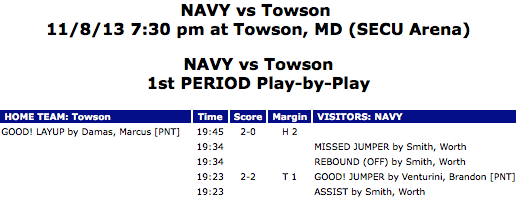
\includegraphics[height = 0.9 in]{pbp_2013.png}
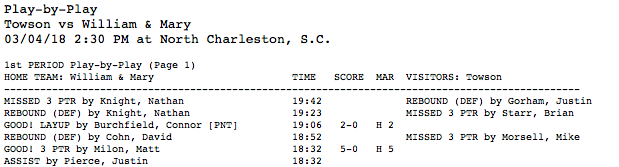
\includegraphics[height = 0.9 in]{pbp_2017.png}
\caption{The table on the left is a sample of play-by-play statistics from the 2013-2014 season; the table on the right is of that of the 2017-2018 season.}
\label{f: pbp}
\end{center}
\end{figure}
\vspace{-23pt}
Statistics from the 2013-2014 season are placed in tables constructed using the code required to make a table in HTML (i.e., HTML-formatted tables), which makes data extraction relatively easy. Statistics from the 2017-2018 season are in text-formatted tables, which makes data extraction difficult. Because of the work I put into the project this past summer, I have completed code for data extraction from the latter, more difficult format. One of the first tasks to complete for spring 2019 is to extract data from HTML-formatted tables. Once all play-by-play data is retrieved, I can place them into a spreadsheet-like data structure called a dataframe. 

Each dataframe corresponds to a single game and consists of time at which an event occurs, the order in which a series of events occur, and the players associated with each event. Figure \ref{f: tree} shows the possibilities for a series of events in the form of a tree diagram.

\begin{figure}[h]
\begin{center}
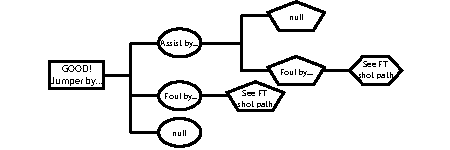
\includegraphics{good_jumper_pbp_final.pdf}
\caption{This tree demonstrates the possible series of events after a successful jump shot attempt. Entries with "null" indicate the end of a series of events.}
\label{f: tree}
\end{center}
\end{figure}
\vspace{-23pt}
A tree diagram helps humans understand how a computer thinks when analyzing this data. In this tree, each branch and shape represents the order in which an event can occur. For example, consider the following series of events in this manner: an assisted good jumper (shot: primary, assist: secondary), followed by a foul (tertiary), and one good free throw (quaternary). Once all play-by-play data have been placed into a dataframe, I can apply clustering algorithms and topology.

A clustering algorithm will allow me to group data with similar traits. Once the clustering is completed, I can apply topological techniques introduced by Dr.~Gunnar Carlsson to understand which parameters have the greatest influence when grouped together. This is done with the understanding that there is not just one type of grouping of parameters. Topological data analysis highlighted by Carlsson will allow us to extract those types.

Topology has proven to be a very useful tool in precision medicine; it was used in the discovery of subgroups of Type 2 diabetes. In this study, researchers used a topological approach to construct a precision model to characterize the complexity of Type 2 diabetes patient populations based on electronic medical records and genotype data (Li et al., 2015). This study found strong similarities among different subgroups of Type 2 diabetes from high-dimensional relationships that could not be observed by hand, such as laboratory tests (Li et al., 2015). Once patients were distinguished into subgroups, statistical methods were applied to clarify treatment options and sources of the disease for each subgroup (Li et al., 2015). Ultimately, three subgroups of Type 2 diabetes were found using the model, suggesting the idea that more than two types of diabetes exist (Li et al., 2015).

In the context of this project, I plan to identify similarities which are not apparent in one- or two-dimensions between different players and lineups that have historically made the team successful in a game. The intention is not to consider high-performing players as a single type, but to consider the best lineup combinations to optimize the team's chances of winning games. 

By using one model, different statistics are blurred together into one model, which can obscure relationships. Topological data analysis provides an algorithm that identifies statistics that have a major impact, including those that seem insignificant to an outcome. When the problem addressed in this project is approached from statistical means, there are powerful tools in statistics for finding the variables with the most explanatory power. However, there are situations where topological data analysis will find features from the data that statistics will be unable to see. This is because statistics has to start from a single model, whereas topological analysis suggests a model. For example, topological data analysis will allow me to construct a model to understand if there is a similarity between one player's rebounding ability and another player's shooting ability.
 
Ultimately, by showing how topology can be applied to sports analytics, I can show how topology can be applied to a wider range of studies and what ideas topology can suggest from discrete data.

\medskip

References
\begin{enumerate}[noitemsep]
\item Carlsson, G. (2009). Topology and Data. \textit{Bulletin of the American Mathematical Society, 46}(2), 255-308.
\item Leonhardt, D. (2003). Pro Basketball; Mavericks’ New Math May Be an Added Edge. \textit{The New York Times}. Retrieved from https://www.nytimes.com/2003/04/27/sports/pro-basketball-mavericks-new-math-may-be-an-added-edge.html
\item Li, L., Cheng, W. Y., Glicksberg, B. S., Gottesman, O., Tamler, R. Chen, R., ... \& Dudley, J.T. (2015). Identification of type 2 diabetes subgroups through topological
analysis of patient similarity. \textit{Science translational medicine, 7}(311), 311ra174.
\item Thamel, P. (2013). Butler has found secret weapon in statistical guru Drew Cannon. \textit{Sports Illustrated}. Retrieved from https://www.si.com/college-basketball/2013/03/20/drew-cannon-butler
\end{enumerate}

\end{document}